\documentclass[journal,12pt,twocolumn]{IEEEtran}

\usepackage{setspace}
\usepackage{gensymb}
\singlespacing
\usepackage[cmex10]{amsmath}

\usepackage{amsthm}

\usepackage{mathrsfs}
\usepackage{txfonts}
\usepackage{stfloats}
\usepackage{bm}
\usepackage{cite}
\usepackage{cases}
\usepackage{subfig}

\usepackage{longtable}
\usepackage{multirow}

\usepackage{enumitem}
\usepackage{mathtools}
\usepackage{steinmetz}
\usepackage{tikz}
\usepackage{circuitikz}
\usepackage{verbatim}
\usepackage{tfrupee}
\usepackage[breaklinks=true]{hyperref}
\usepackage{graphicx}
\usepackage{tkz-euclide}

\usetikzlibrary{calc,math}
\usepackage{listings}
    \usepackage{color}                                            %%
    \usepackage{array}                                            %%
    \usepackage{longtable}                                        %%
    \usepackage{calc}                                             %%
    \usepackage{multirow}                                         %%
    \usepackage{hhline}                                           %%
    \usepackage{ifthen}                                           %%
    \usepackage{lscape}     
\usepackage{multicol}
\usepackage{chngcntr}

\DeclareMathOperator*{\Res}{Res}

\renewcommand\thesection{\arabic{section}}
\renewcommand\thesubsection{\thesection.\arabic{subsection}}
\renewcommand\thesubsubsection{\thesubsection.\arabic{subsubsection}}

\renewcommand\thesectiondis{\arabic{section}}
\renewcommand\thesubsectiondis{\thesectiondis.\arabic{subsection}}
\renewcommand\thesubsubsectiondis{\thesubsectiondis.\arabic{subsubsection}}
\newtheorem{theorem}{Theorem}[section]
\newtheorem{corollary}{Corollary}[theorem]
\newtheorem{lemma}[theorem]{Lemma}
\newtheorem{definition}{Definition}[section]


\hyphenation{op-tical net-works semi-conduc-tor}
\def\inputGnumericTable{}                                 %%

\lstset{
%language=C,
frame=single, 
breaklines=true,
columns=fullflexible
}
\begin{document}

\newcommand{\BEQA}{\begin{eqnarray}}
\newcommand{\EEQA}{\end{eqnarray}}
\newcommand{\define}{\stackrel{\triangle}{=}}
\bibliographystyle{IEEEtran}
\raggedbottom
\setlength{\parindent}{0pt}
\providecommand{\mbf}{\mathbf}
\providecommand{\pr}[1]{\ensuremath{\Pr\left(#1\right)}}
\providecommand{\qfunc}[1]{\ensuremath{Q\left(#1\right)}}
\providecommand{\sbrak}[1]{\ensuremath{{}\left[#1\right]}}
\providecommand{\lsbrak}[1]{\ensuremath{{}\left[#1\right.}}
\providecommand{\rsbrak}[1]{\ensuremath{{}\left.#1\right]}}
\providecommand{\brak}[1]{\ensuremath{\left(#1\right)}}
\providecommand{\lbrak}[1]{\ensuremath{\left(#1\right.}}
\providecommand{\rbrak}[1]{\ensuremath{\left.#1\right)}}
\providecommand{\cbrak}[1]{\ensuremath{\left\{#1\right\}}}
\providecommand{\lcbrak}[1]{\ensuremath{\left\{#1\right.}}
\providecommand{\rcbrak}[1]{\ensuremath{\left.#1\right\}}}
\theoremstyle{remark}
\newtheorem{rem}{Remark}
\newcommand{\sgn}{\mathop{\mathrm{sgn}}}
\providecommand{\abs}[1]{\vert#1\vert}
\providecommand{\res}[1]{\Res\displaylimits_{#1}} 
\providecommand{\norm}[1]{\lVert#1\rVert}
%\providecommand{\norm}[1]{\lVert#1\rVert}
\providecommand{\mtx}[1]{\mathbf{#1}}
\providecommand{\mean}[1]{E[ #1 ]}
\providecommand{\fourier}{\overset{\mathcal{F}}{ \rightleftharpoons}}
%\providecommand{\hilbert}{\overset{\mathcal{H}}{ \rightleftharpoons}}
\providecommand{\system}{\overset{\mathcal{H}}{ \longleftrightarrow}}
	%\newcommand{\solution}[2]{\textbf{Solution:}{#1}}
\newcommand{\solution}{\noindent \textbf{Solution: }}
\newcommand{\cosec}{\,\text{cosec}\,}
\providecommand{\dec}[2]{\ensuremath{\overset{#1}{\underset{#2}{\gtrless}}}}
\newcommand{\myvec}[1]{\ensuremath{\begin{pmatrix}#1\end{pmatrix}}}
\newcommand{\mydet}[1]{\ensuremath{\begin{vmatrix}#1\end{vmatrix}}}
\numberwithin{equation}{subsection}
\makeatletter
\@addtoreset{figure}{problem}
\makeatother
\let\StandardTheFigure\thefigure
\let\vec\mathbf
\renewcommand{\thefigure}{\theproblem}
\def\putbox#1#2#3{\makebox[0in][l]{\makebox[#1][l]{}\raisebox{\baselineskip}[0in][0in]{\raisebox{#2}[0in][0in]{#3}}}}
     \def\rightbox#1{\makebox[0in][r]{#1}}
     \def\centbox#1{\makebox[0in]{#1}}
     \def\topbox#1{\raisebox{-\baselineskip}[0in][0in]{#1}}
     \def\midbox#1{\raisebox{-0.5\baselineskip}[0in][0in]{#1}}
\vspace{3cm}
\title{ EE3900 : Quiz-2}
\author{Nelakuditi Rahul Naga - AI20BTECH11029}
\maketitle
\newpage
\bigskip
\renewcommand{\thefigure}{\theenumi}
\renewcommand{\thetable}{\theenumi}
Download all python codes from 
\begin{lstlisting}
https://github.com/Rahul27n/EE3900/blob/main/Quiz_2/Quiz_2.py
\end{lstlisting}
%
and all latex-tikz codes from 
%
\begin{lstlisting}
https://github.com/Rahul27n/EE3900/blob/main/Quiz_2/Quiz_2.tex
\end{lstlisting}
\vspace{0.5cm}
\section{QUESTION: 3.19(b)}
For the following pair of input $z$-transform $X(z)$ and system function $H(z)$ determine the region of convergence for the output $z$-transform $Y(z)$:
\begin{align}
X(z) &= \frac{1}{1-2z^{-1}}, \quad \abs{z} < 2 \nonumber \\
H(z) &= \frac{1}{1-\frac{1}{3}z^{-1}}, \quad \abs{z} > \frac{1}{3} \nonumber
\end{align}
\section{SOLUTION}
We know that if $X(z) = \frac{1}{1-az^{-1}}$ :
\begin{align}
x[n]=  
\begin{cases}
a^{n}u[n], & \text{if } \abs{z} > \abs{a} \\
-a^{n}u[-n-1], & \text{if } \abs{z} < \abs{a} \nonumber
\end{cases}
\end{align}
Therefore we have :
\begin{align}
x[n] &= -2^{n}u[-n-1] \\
h[n] &= \Bigg(\frac{1}{3}\Bigg)^{n}u[n]
\end{align}
The $z$- transform expansion of $x[n]$ is given by:
\begin{align}
X(z) &= \sum_{n=-\infty}^{\infty}x[n]z^{-n} \\
&= \sum_{n=-\infty}^{-1}2^{n}z^{-n} \\
&= \sum_{m=1}^{\infty}\Bigg(\frac{z}{2}\Bigg)^{m}
\end{align}
Clearly the above geometric series converges only when we have :
\begin{align}
\abs{2^{-1}z} < 1 \implies \abs{z} < 2 \label{eq:1}
\end{align}
Therefore the ROC of $x[n]$ is given by \eqref{eq:1}.

The $z$- transform expansion of $h[n]$ is given by:
\begin{align}
H(z) &= \sum_{n=-\infty}^{\infty}h[n]z^{-n} \\
&= \sum_{n=0}^{\infty}\Bigg(\frac{1}{3}\Bigg)^{n}z^{-n} \\
&= \sum_{n=0}^{\infty}\Bigg(\frac{1}{3z}\Bigg)^{n}
\end{align}
Clearly the above geometric series converges only when we have :
\begin{align}
\abs{3z} > 1 \implies \abs{z} > \frac{1}{3} \label{eq:2}
\end{align}
Therefore the ROC of $h[n]$ is given by \eqref{eq:2}.

We know from the convolution theorem that :
\begin{align}
Y(z) &= X(z)H(z) \\
Y(z) &= \frac{1}{(1-2z^{-1})({1-\frac{1}{3}z^{-1})}} \\
Y(z) &= \frac{3z^{2}}{(z-2)(3z-1)}
\end{align}

We also know that :
\begin{align}
R_{x_{1}[n]*x_{2}[n]} &= R_{x_1[n]} \cap R_{x_2[n]}
\end{align}
where $R_{x[n]}$ represents the ROC of $X(z)$.

We have :
\begin{align}
y[n] &= x[n]*h[n]
\end{align}
Therefore from \eqref{eq:1} and \eqref{eq:2} the ROC of $Y(z)$ is given by:
\begin{align}
R_{y[n]} &= \frac{1}{3} < \abs{z} < 2
\end{align}

The plots of $x[n]$ , $h[n]$ and the ROC of $Y(z)$ are given by:
\begin{figure}[!ht]
    \centering
    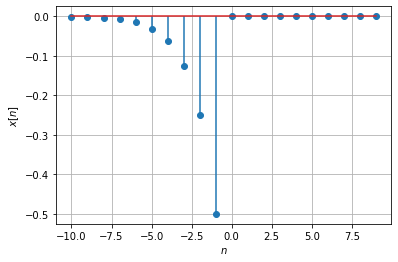
\includegraphics[width=\columnwidth]{Quiz_2_Fig_1.png}
    \caption{$x[n]$}
    \label{x[n]}
\end{figure}

\begin{figure}[!ht]
    \centering
    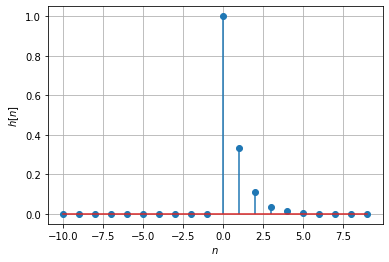
\includegraphics[width=\columnwidth]{Quiz_2_Fig_2.png}
    \caption{$h[n]$}
    \label{h[n]}
\end{figure}

\begin{figure}[!ht]
    \centering
    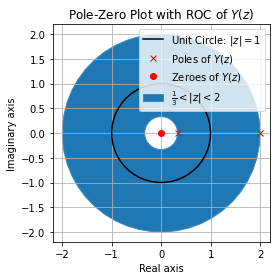
\includegraphics[width=\columnwidth]{Quiz_2_Fig_3.png}
    \caption{ROC of $Y(z)$}
    \label{ROC of Y(z)}
\end{figure}
\end{document}

